[71~r\textsuperscript{o}] oriretur; ideo supputata lunae\protect\index{Sachverzeichnis}{luna} parallaxi\protect\index{Sachverzeichnis}{parallaxis} corrigendus est ejus locus, indagandumque quo in loco sit nunc apparitura, si ex ipso terrae centro vel alio loco cui verticalis est, spectetur. Parallaxis\protect\index{Sachverzeichnis}{parallaxis} autem seu error tanto major est, quanto major obliquitas anguli quem facit ad horizontem, seu quanto minor elevatio. Sed correctio hujus erroris est in potestate, tum quia anguli  obliquitas observatione data est, tum quia altitudinem Lunae\protect\index{Sachverzeichnis}{luna}, et semidiametrum terrae satis explorata habemus. Esto Horizon loci \textit{acb} ad cujus centrum \textit{c} radius lunae\protect\index{Sachverzeichnis}{luna} \textit{cd} facit angulum observatione cognitum \textit{dcb}. Esto centrum terrae \textit{e} ducaturque linea a centro terrae ad Lunam\protect\index{Sachverzeichnis}{luna} \textit{ed}.
   %\begin{wrapfigure}{l}{0.5\textwidth}                    
   %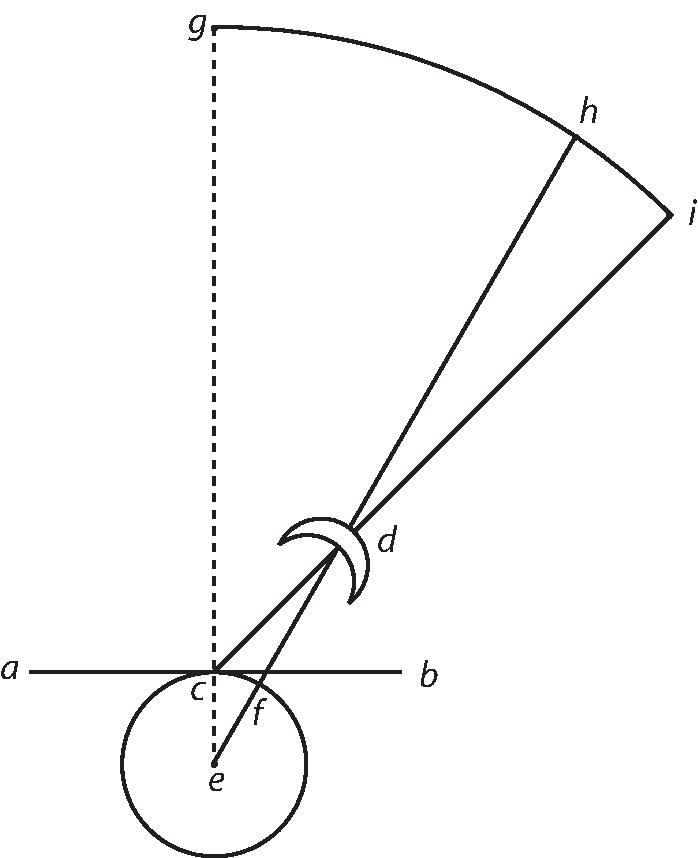
\includegraphics[width=0.5\textwidth]{images/35_15_6_71rfig1}
   %\\\centering\textit{[Fig. 1]}
   %\end{wrapfigure}
Constat in Triangulo \textit{dec} cognitum esse angulum \edtext{unum}{\lemma{}\Afootnote{unum \textit{ erg.} \textit{ L}}} \textit{dce} compositum ex angulo cognito \textit{dcb} et recto \textit{bce} et \edtext{cognita esse}{\lemma{}\Afootnote{cognita esse \textit{ erg.} \textit{ L}}} latera \edtext{duo}{\lemma{}\Afootnote{duo \textit{ erg.} \textit{ L}}}: \textit{ec} semidiametrum terrae, et \textit{ed} distantiam Lunae\protect\index{Sachverzeichnis}{luna} a centro terrae. Ergo per canones trigonometricos etiam \edtext{unum}{\lemma{}\Afootnote{unum \textit{ erg.} \textit{ L}}} residuum latus \textit{cd} et \edtext{duo}{\lemma{}\Afootnote{duo \textit{ erg.} \textit{ L}}} residui anguli \textit{cde} et \textit{ced} cognoscentur, et cognito angulo \textit{ced} cognoscetur arcus \textit{cf} in terra et ei \edtext{respondens in circulo magno}{\lemma{respondens}\Afootnote{ \textit{ (1) }\ magno in circulo \textit{ (2) }\ in circulo magno \textit{ L}}} sphaerae coelestis arcus \textit{gh} ex centro terrae \textit{e} et Zenith loci \textit{g} in sphaera coelesti sumpto descriptus, (ac proinde  portio cujusdam verticalis \edtext{loci) et, si}{\lemma{loci)}\Afootnote{ \textit{ (1) }\ etsi \textit{ (2) }\ et, si \textit{ L}}} continuetur, per locum Lunae\protect\index{Sachverzeichnis}{luna} incorrectum \textit{i} in eadem sphaera assumptum transiens. Unde intelligitur, \textit{h} esse in sphaera coelesti locum Lunae\protect\index{Sachverzeichnis}{luna} verum. Hinc \textso{Tabulae} construi poterunt, quibus data Lunae\protect\index{Sachverzeichnis}{luna} obliquitate seu elevatione \edtext{super horizontem}{\lemma{}\Afootnote{super horizontem \textit{ erg.} \textit{ L}}}, quantitas parallaxeos\protect\index{Sachverzeichnis}{parallaxis} sine calculo inveniatur. Idem Mechanice, sine tabula et calculo, \textso{instrumento} apto, poterit praestari. Habemus ergo veram \textso{Lunae}\protect\index{Sachverzeichnis}{luna} \textso{latitudinem }\protect\index{Sachverzeichnis}{latitudo}hac observatione inventam, et in sphaera artificiali notandam.\pend \pstart Ego vero hoc amplius ajo ex eadem observatione \textso{Tempus praesens Mundi} elici posse.\pend \clearpage
   \hspace{0.5ex}
   \begin{center}
   %\begin{wrapfigure}{l}{0.45\textwidth}                    
   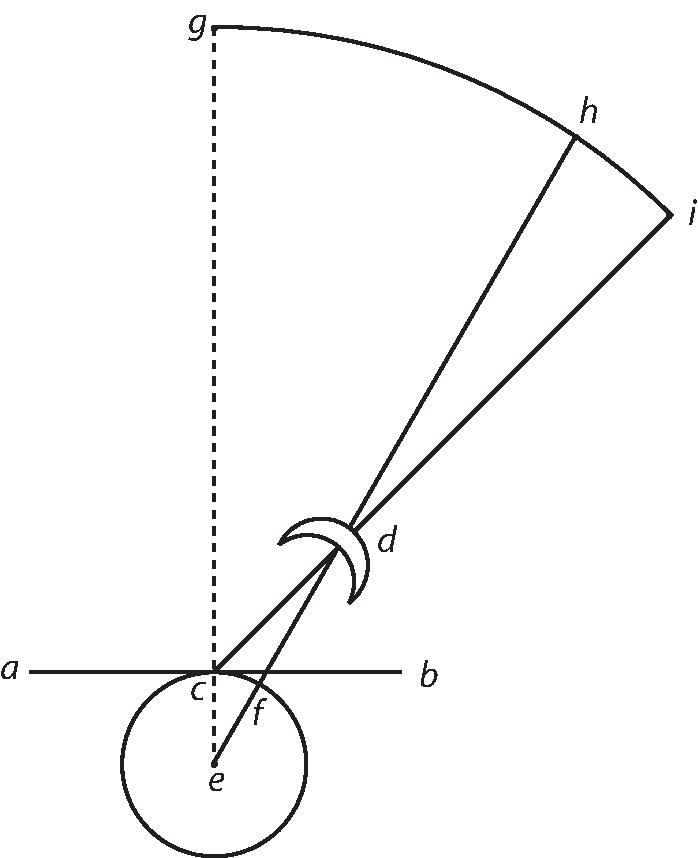
\includegraphics[width=0.45\textwidth]{images/35_15_6_71rfig1}
   \\\centering\textit{[Fig. 1]}
   %\end{wrapfigure}
   \end{center}
 \pstart 